\section{Discussion}\label{sec:discussion}
\subsection{Survey Sensitivity}
\label{sec:sensitivity}
The required power for a certain extra terrestrial intelligent (ETI) transmitter to be detected depends on its directionality and other signal characteristics. 
%For all three signal types, w
We can measure the transmitter power of an ETI beacon in terms of the effective isotropic radiated power (EIRP; \citealt{Enriquez:2017}) as,
\begin{equation}
%    {\rm EIRP} = \sigma \times {4 \pi d_\star^2} \frac{\rm SEFD_{\rm HBA}}{\delta{\nu}_{t}} \sqrt{\frac{\delta{\nu}}{n_{p}t_{obs}{\omega}}}  \>\> W/Hz,
    {\rm EIRP} = \sigma \times {4 \pi d_\star^2} \;\frac{{\rm SEFD}}{\delta{\nu_t}}\sqrt{\frac{\delta{\nu}}{n_{p}t_{obs}}}  \>\> \mathrm{W}\;
    \label{Eq:EIRP}
\end{equation}
Here, $\sigma$ is the required S/N, $\delta{\nu}$ is the bandwidth of the received signal, 
$\delta{\nu}_{t}$ is the transmitted bandwidth, $t_{obs}$ is the observing integration time, SEFD is the System Equivalent Flux Density, $n_p$ is the number of polarizations, 
%\omega$ is the duty cycle of the signal, 
and $d_\star$ is the distance between the transmitter and the receiver, i.e., the distance to the star. We considered $\delta{\nu}_{t}$ to be 1\,Hz. For the narrowband signals we consider in our Doppler searches, we assume $\delta{\nu}$ is matched to our spectral resolution and further assume a temporal duty cycle of $100\%$.
%$\omega$ is assumed to be 100\% and $\delta{\nu}$ and $\delta{\nu}_{t}$ is $2.98$~Hz as per our observing specifications.
%are assumed to be 3Hz. For PSM signals, we assumed the narrowest wide-band signal to be 3 kHz and $\omega$ to be 10\%. For the broadband aDM transients signals, we assumed $\delta{\nu}$ and $\delta{\nu}_{t}$ is assumed to be 80 MHz and $t_{obs}$ is assumed to be 1 msec. \\
%The measured SEFD of the international HBA stations used in this survey is between 120 MHz and 180 MHz, is around 2 kJy, and increases significantly up to 12 kJy at 240 MHz. 

The SEFD of the international HBA stations used in this survey is on average $\sim 900$~Jy for most of the band, rising to $\sim 1.2$~kJy at the band edges~\citep{2013arXiv1305.3550V}. For reference, the SEFD of the GBT at the $1.4$~GHz is around 10 Jy. This difference in sensitivity is 
%due in small to the larger collecting area of the GBT and the cooled analogue front-end, but primarily 
because sky temperature scales as $\nu^{-2.6}$ meaning it can be hundreds of times higher in the LOFAR band. However, the average values are of little use as there is also a large degree of variation in the sky temperature across the sky. For this reason, we perform a separate calculation for every target to determine the relevant luminosity limit in each case.  For example, the sensitivity to each off-boresight target is determined by its proximity to the pointing coordinates. Figure \ref{fig:off_beam_sens} depicts both the impact on sensitivity and the number of background stars within a given LOFAR beam. Figure \ref{fig:inbeam_trgts_SDSS} shows an example pointing from the survey and also well illustrates the vast volume of targets that appear in a LOFAR beam (pink).


Figure \ref{fig:Cumulative_EIRP_plots} presents the luminosity limits for the cumulative targets of this survey within the frequency range of $110-190$ MHz. In this figure, the limiting luminosity is compared to notable values of Equivalent Isotropic Radiated Power (EIRP) for various scenarios. These scenarios include a Kardashev I type advanced civilization transmitting at a power level of $10^{17}$ W, an advanced civilization producing planetary radar-level transmissions with a transmitting power of $10^{13}$ W, and a cumulative aircraft radar-type system transmitted across a large solid angle with a power of $10^{10}$ W \citep{Siemion_KEPLER_ApJ}. The Figure demonstrates that due to the varying system temperature ($T_{sys}$) across the frequency band, our observations were sensitive to detecting a range of Kardashev I type targets. Specifically, we were able to detect approximately 25\% of the targets at the lower end of the frequency band, increasing to nearly 80\% of the targets at the higher end of the band.

\begin{figure*}
  % \gridline{\fig{figures/EIRP_plots/Dist_EIRP_cuml.pdf}{0.46\textwidth}{(a)}
  %           \fig{figures/EIRP_plots/EIRP_cummulative_plot.pdf}{0.46\textwidth}{(b)}
  %           }
  \centering
     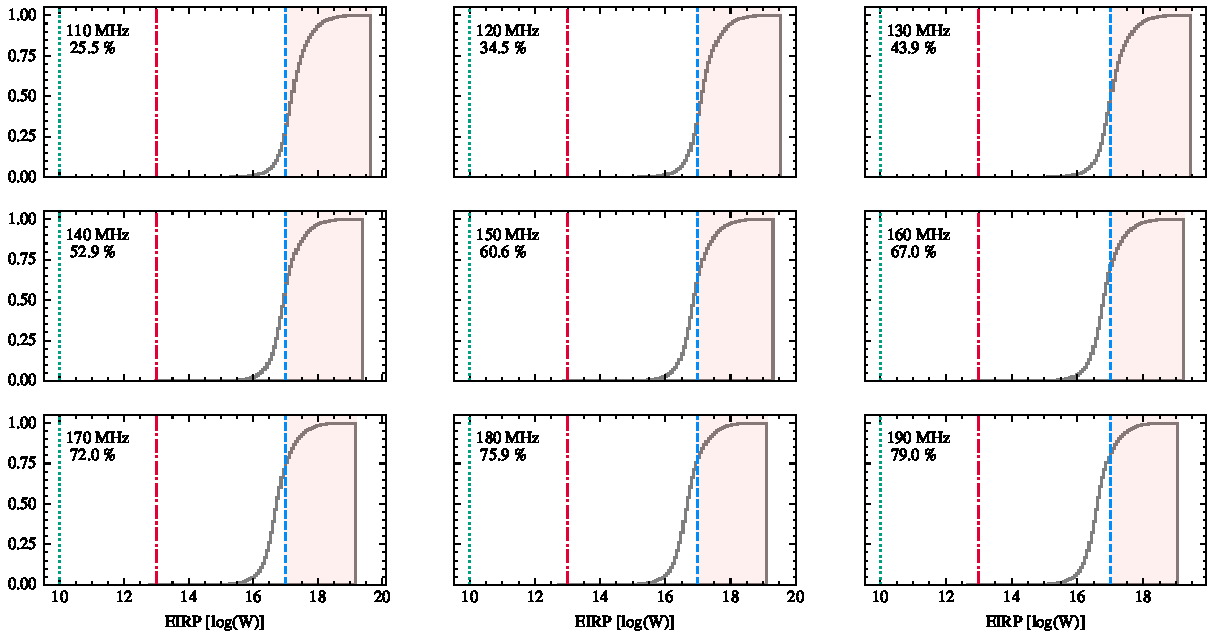
\includegraphics[width = \textwidth]{SETI/figures/EIRP_plots/EIRP_hist_plot.pdf}
      \caption{Cumulative histogram of EIRP limits of this survey across the HBA band. Reference luminosities for three civilization levels emitting $10^{17}$, $10^{13}$ or $10^{10}$~W are shown in blue, red and green respectively. The percentage of targets where the station is sensitive to the transmission of $10^{17}$~W is shown, as a function of frequency across the band. At lower frequencies sensitivity to $10^{17}$ emitters drops off as the $T_{sys}$ rises. The $\bar T_{sys}$ varies from 1260 K down to 322 K as frequency is increased across the band. Detailed calculations are presented in Appendix B.}
  \label{fig:Cumulative_EIRP_plots}
\end{figure*}


\subsection{Starlink Interference}
A recent study by \cite{LOFAR-Starlink} has shown that unintended electromagnetic radiation (UEMR) from the Starlink satellite constellation produced broadband interference ranging from 0.1 to 10 Jy and narrowband interference ranging from 10 to 500 Jy. UEMR was detected at frequencies at 110 to 188 MHz, which is the bandwidth of the HBA used in this study. UEMR has many potential consequences for low frequency radio observations. Analysis of \verb|turboSETI| hit detection's within 1 MHz the UEMR narrowband emission frequencies (125, 135, 143, 150, 175 MHz; \citealt{LOFAR-Starlink}) show that 17.8\% of total detected hits are within this region. This region occupies 18.5\% of this study's bandwidth. This result is expected, as UEMR affects a number of different types of radio searches, it does not affect narrowband searches of this nature. This is due to two factors. Firstly satellites in Low Earth Orbit (LEO) to Geostationary orbit (GEO) usually have velocities that are too high for them to be detected with the temporal resolution of our data, and they are at drift rate values outside the parameters of this search ($>$4 Hz/s). Secondly, the satellites are in the near field of each station's beam and due to their relative distance to the observer compared to the bore sight target a satellite less likely to appear in both beams simultaneously. It is concluded that the Starlink constellation does not add to the number of narrowband hits detected in this study.


\subsection{Figure of Merit}
To compare SETI surveys, \cite{Enriquez:2017} introduced a figure of merit known as the Continuous Waveform Transmitter Rate (CWTFM), 

\begin{equation}
    \text{CWTFM} = \zeta_{\text{AO}} \dfrac{\text{EIRP}}{N_{\text{stars}} \nu_{\text{rel}}}
    \label{eq:CWTFM}
\end{equation}

Where $N_{\text{stars}}$ is the number of stars in each pointing for a given survey, $\nu_{\text{rel}}$ is the fractional bandwidth of the survey, $\Delta \nu_{\text{tot}}/\nu_{\text{mid}}$ where $\nu_{\text{mid}}$ is the central frequency of the survey. $\zeta_{\text{AO}}$ is the normalization factor such that $\text{CWTFM} = 1$ and the EIRP is equal to the Arecibo radio telescope's S-band planetary radar, if it were transmitted across a whole hemisphere, $(\sim 10^{13}$~W~\citealt{Siemion_KEPLER_ApJ}). In \Cref{fig:EIRP_compare}, we compare our results to those from some other SETI surveys. As this survey continues, the transmitter rate will decrease with the volume of stars observed $(N_\text{stars})$, as outlined by \Cref{eq:transmitter_rate}.

 \begin{equation}
     \text{Transmitter Rate} = \log \left[ \dfrac{1}{N_{\text{stars}} \cdot \nu_{\text{rel}}} \right]
     \label{eq:transmitter_rate}
 \end{equation}

As dictated by \Cref{Eq:EIRP} to be sensitive to lower powered ETI transmitters, the observation sensitivity needs to be greater. This can be done by employing further LOFAR stations for $n$-site simultaneous observations through coherent summation.
 
\begin{figure*}
    \centering
    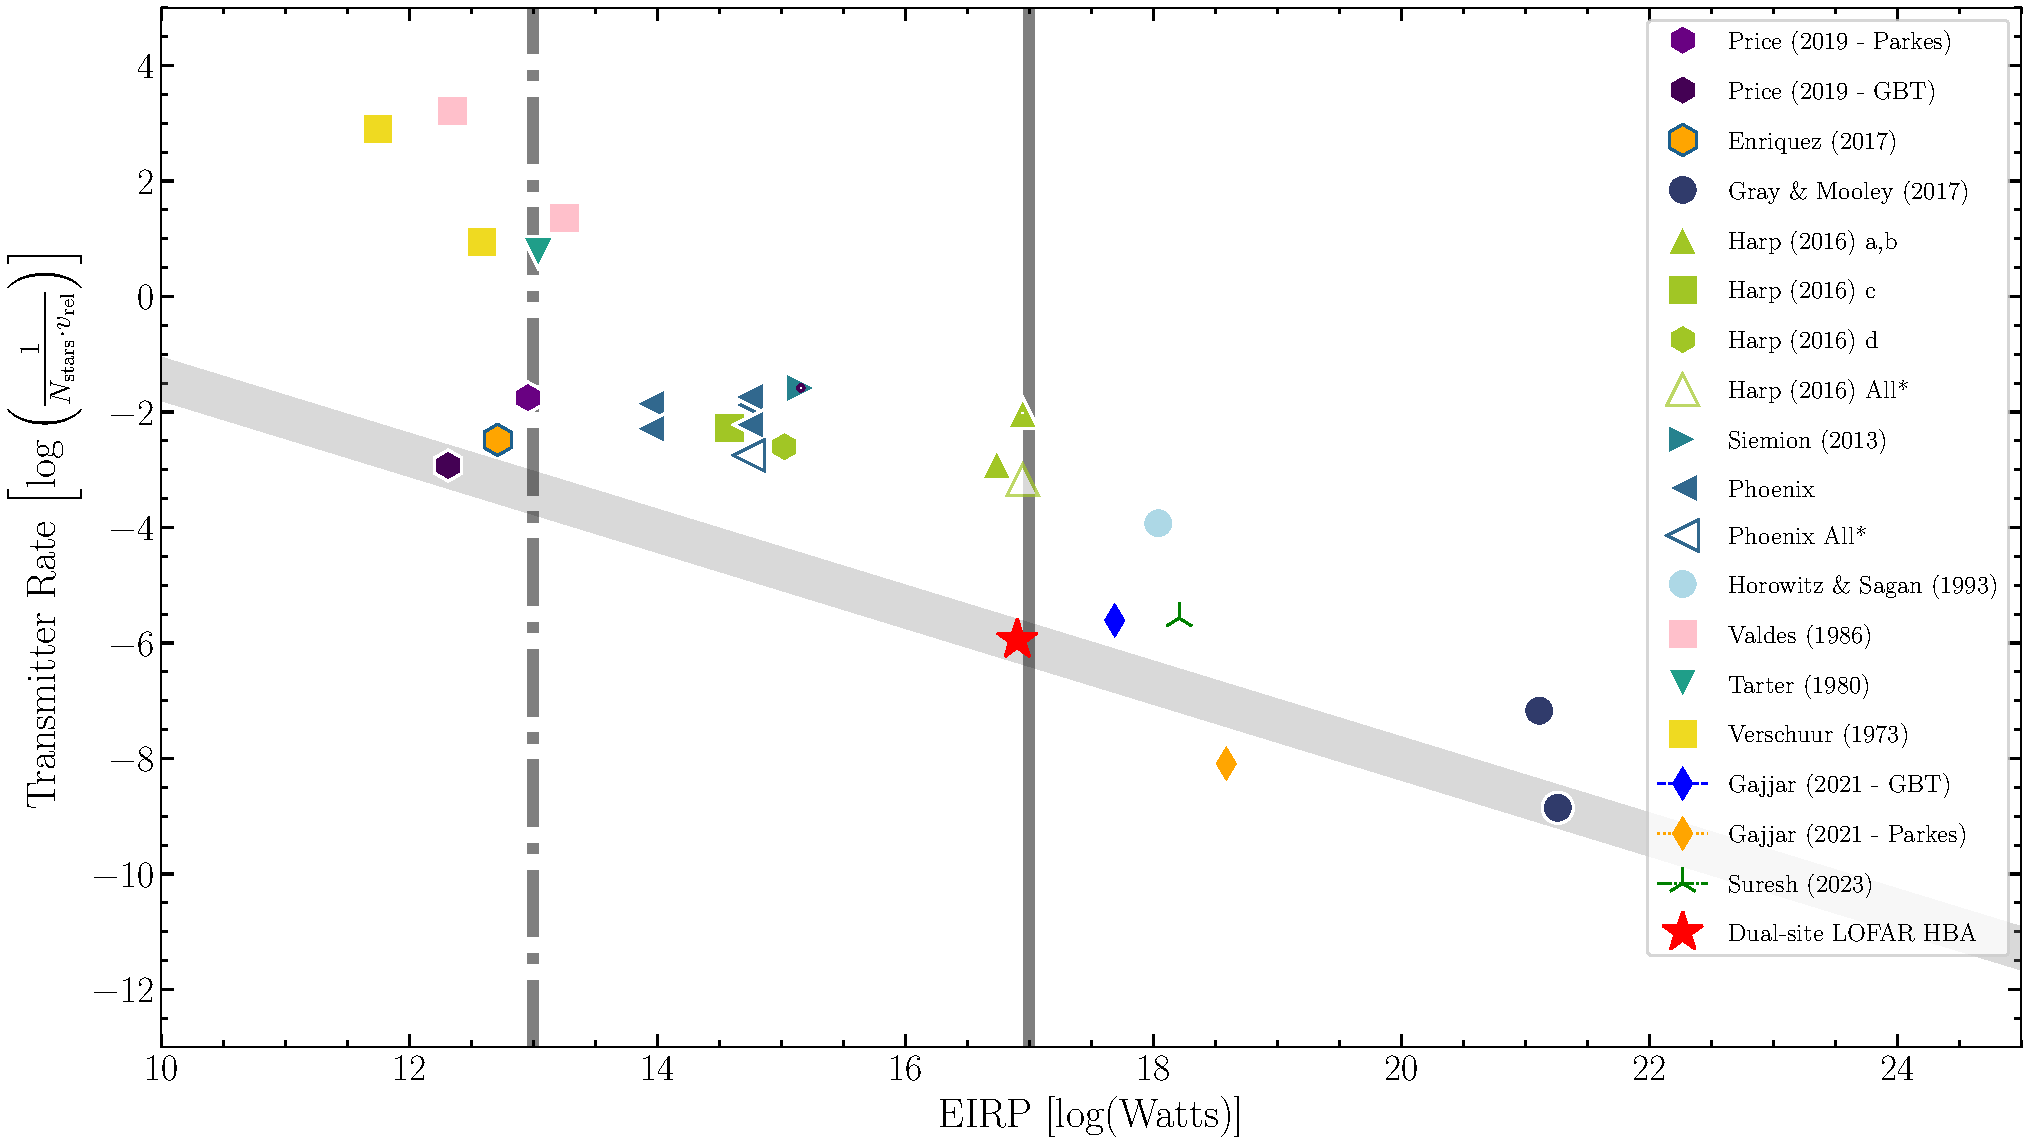
\includegraphics[width=\linewidth]{SETI/figures/SETI_limits_comparison.pdf}
    \caption{Comaprison of our study (highlighted in red) to prior surveys. The plot presents the transmitter rate versus Effective Isotropic Radiated Power (EIRP), with the grey line indicating the transmitter rate as a function of EIRP. A solid vertical grey line illustrates the energy surplus of a Kardashev Type-I civilization. Additionally, a dotted-dashed grey line depicts the EIRP of the Arecibo planetary radar. The gray thick line shows the slope
    of the transmitter-rate as a function of their EIRP power.  Distance used for EIRP calculation is $\bar d + d_\sigma = 7009 \; \text{ly}$.
    \label{fig:EIRP_compare}}
\end{figure*}

% \subsection{Where does this leave us?}
\subsection{110 - 190 MHz Technosignature Parameter Space}
 The number of intelligent civilizations is quantified using \Cref{eq:Drake_equation}, coined by \cite{Drake:1961bv}. 
\begin{equation}
    N = R_* f_p N_e f_l f_i f_c L 
    \label{eq:Drake_equation}
\end{equation}
 In this expression $N$ is the number of communicative civilizations in the Milky Way galaxy, $R_{*}$ is the rate of star formation per year in the galaxy, $f_{p}$ is the fraction of stars that have planets around them, $n_{e}$ is the average number of planets that can potentially support life per star that has planets, $f_{l}$ is the fraction of potentially life-supporting planets that actually develop life, $f_{i}$ is the fraction of planets with life that go on to develop intelligent life and $f_{c}$ is the fraction of civilizations that develop a technology that releases detectable signs of their existence into space. \\ 

In \cite{2022VishalPulsed} a modified variation of the Drake equation (Equation. (\ref{eq:modified-drake}); \citealt{Sagan1966}) is used to constrain the fraction of narrowband emitting civilizations $(f_c^n)$.  

\begin{equation}
    N =  R_{\text{IP}}f^n_cL
    \label{eq:modified-drake}
\end{equation}

Here  $R_{\text{IP}}$ is defined as the emergence rate $(\text{yr}^{-1})$ of intelligent life in the Milky Way.  \Cref{fig:SETI-constraint} shows the constraint that this survey places on $f_c^n$ when using a Poisson sided upper limit at 95\% confidence which in this case is 2.995 as per \cite{1986_Poission_tables}. This provides the most strigent constraint of $f^n_c$ in this frequency range.
 % Eq. \ref{eq:Drake_equation} isn't intended to be used for an exact number of civilizations in the Galaxy as every parameter in the equation is largely unconstrained in their own respective right. However, in can provide a broad estimation that lends itself very useful when performing a SETI search.  

\begin{figure}
    \centering
    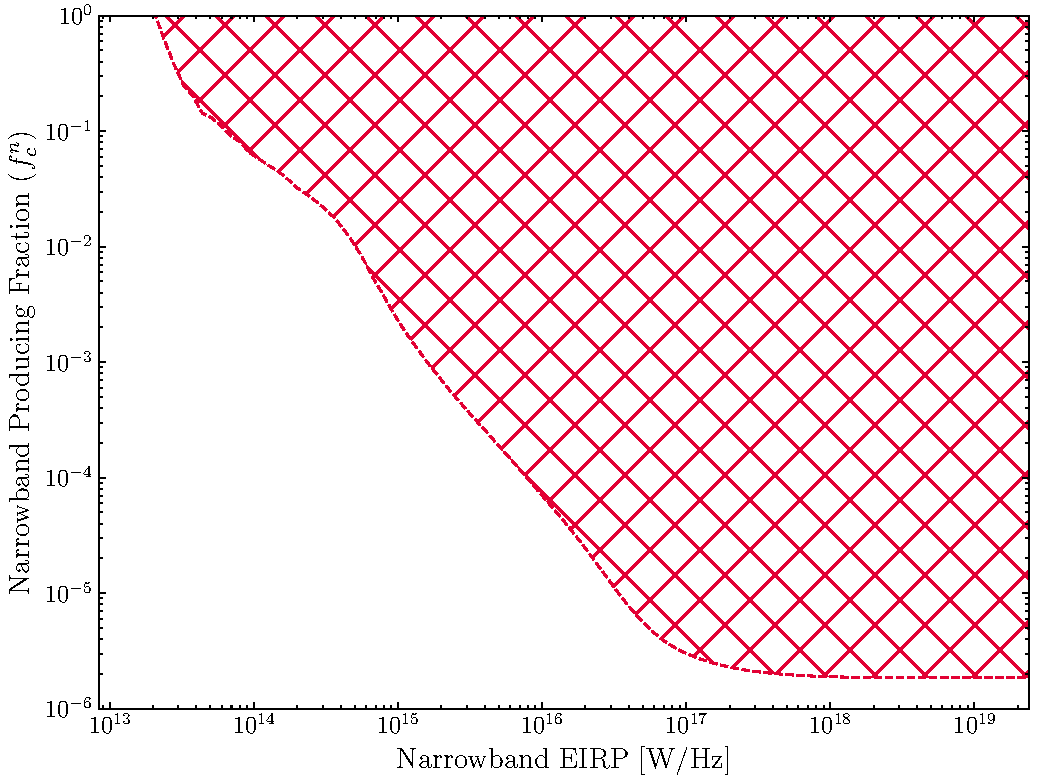
\includegraphics[width = 0.8\textwidth]{SETI/figures/narrowband-fraction.pdf}
    \caption{The fraction of stars that produce narrow-band emission ($f^n_c$) against the transmitter power of the total target pool. The hashed region (red) shows the constraints this survey places on a value of $f^n_c$ at 110 - 190 MHz.}
    \label{fig:SETI-constraint}
\end{figure}

\subsection{Future work using LOFAR 2.0}

LOFAR is soon to undergo a staged series of upgrades across all stations in the array. These upgrades at individual stations across Europe will involve the installation of a new Receiver Control Unit (RCU) as described in \cite{LOFAR2}. These RCUs will enable the simultaneous use of both the LBA and HBA in the frequency range of 15 - 240 MHz. This enhancement will allow for a SETI survey across a broader low-frequency band.

Specifically, at 30 MHz, the FWHM will cover an area of 19.39 deg$^2$, decreasing to 1.73 deg$^2$ at 190 MHz. This will enable follow-up LOFAR surveys to encompass a larger volume of stars and a broader frequency domain.